\vspace{-0.5em}
$$
    P^0 = R_1^0 P^1 + T_1^0
$$
\subsection{Rotations}
    \subsubsection{Rotational Matrix \texorpdfstring{\hfill $R_{x_{i,\theta}}$}{}}
        \vspace{-1em}
        % $$
        % s_\theta \vcentcolon= \sin(\theta) \qquad c_\theta \vcentcolon= \cos(\theta)
        % $$
        $$
        \begin{bmatrix}
            1 & 0 & 0\\
            0 & c_\theta &-s_\theta\\
            0 & s_\theta & c_\theta
        \end{bmatrix}_x
        \quad
        \begin{bmatrix}
            c_\theta &0 & s_\theta\\
            0 & 1 & 0\\
            -s_\theta & 0 & c_\theta
        \end{bmatrix}_y
        \quad
        \begin{bmatrix}
            c_\theta &-s_\theta& 0\\
            s_\theta & c_\theta& 0\\
            0 & 0 & 1
        \end{bmatrix}_z
        $$
        $$
            R^{-1} = R^T \qquad \det(R) = \pm 1
        $$
        %  \subsubsubsection{Properties}
        %     \begin{itemize}
        %         \item orthogonal
        %         \item $R^{-1} = R^T$
        %         \item $\det(R) = \pm 1$
        %     \end{itemize}
    \subsubsection{Composition of Rotations}
        \subsubsubsection{Post Multiply}
            About "new"/ current frame of object:
            \begin{center}
                \resizebox{\linewidth}{!}{
                    \includegraphics[
                        page = {3},
                        trim = {4.9cm, 8.8cm, 5.2cm, 4.7cm}, %left bottom right top
                        clip
                    ]{Spatial_Description/01_2020-09-29_Spatial-Description.pdf}
                }
            \end{center}
        \subsubsubsection{Pre Multiply \hfill "Fixed First"}
            About original/ fixed frame:
            \begin{center}
                \resizebox{\linewidth}{!}{
                    \includegraphics[
                        page = {3},
                        trim = {4.9cm, 2.3cm, 5.2cm, 11.7cm}, %left bottom right top
                        clip
                    ]{Spatial_Description/01_2020-09-29_Spatial-Description.pdf}
                }
            \end{center}
    \subsection{Homogeneous Transformation}
        \subsubsubsection{Principle}
            \vspace{0.5em}
            $$
                y = ax + b, \qquad y = \begin{bmatrix}a&b\end{bmatrix}\begin{bmatrix}x\\1\end{bmatrix}, \qquad \begin{bmatrix}y\\1\end{bmatrix} = \begin{bmatrix}a&b\\0&1\end{bmatrix}\begin{bmatrix}x\\1\end{bmatrix}
            $$
        \subsubsubsection{Application \hfill $H_1^0$}
            \vspace{0.5em}
            $$
                P^0 = R_1^0 P^1 + T_1^0 \quad\longrightarrow\quad P_H^0 = H_1^0 P_H^1
            $$
            $$
               \begin{bmatrix} P^0\\1 \end{bmatrix} = \underbrace{\begin{bmatrix} R_1^0 & T_1^0\\ [0] &1 \end{bmatrix}}_{H_1^0} \begin{bmatrix} P^1\\1 \end{bmatrix}
            $$
            {\small $T_1^0$: Translation from 0 to 1}
        \subsubsubsection{Inverse \hfill $\left(H_1^0\right)^{-1}$}
            \vspace{0.5em}
            $$
                \left(H_1^0\right)^{-1} = H_0^1 = \begin{bmatrix}
                    \left(R_1^0\right)^T & -\left(R_1^0\right)^T T_1^0\\[.5em]
                    [0] & 1
                \end{bmatrix}
            $$
            

        